%!TeX root=../pridetop.tex
\chapter[Chapter \thechapter]{}
	
	\begin{figure}[t!]
\centering
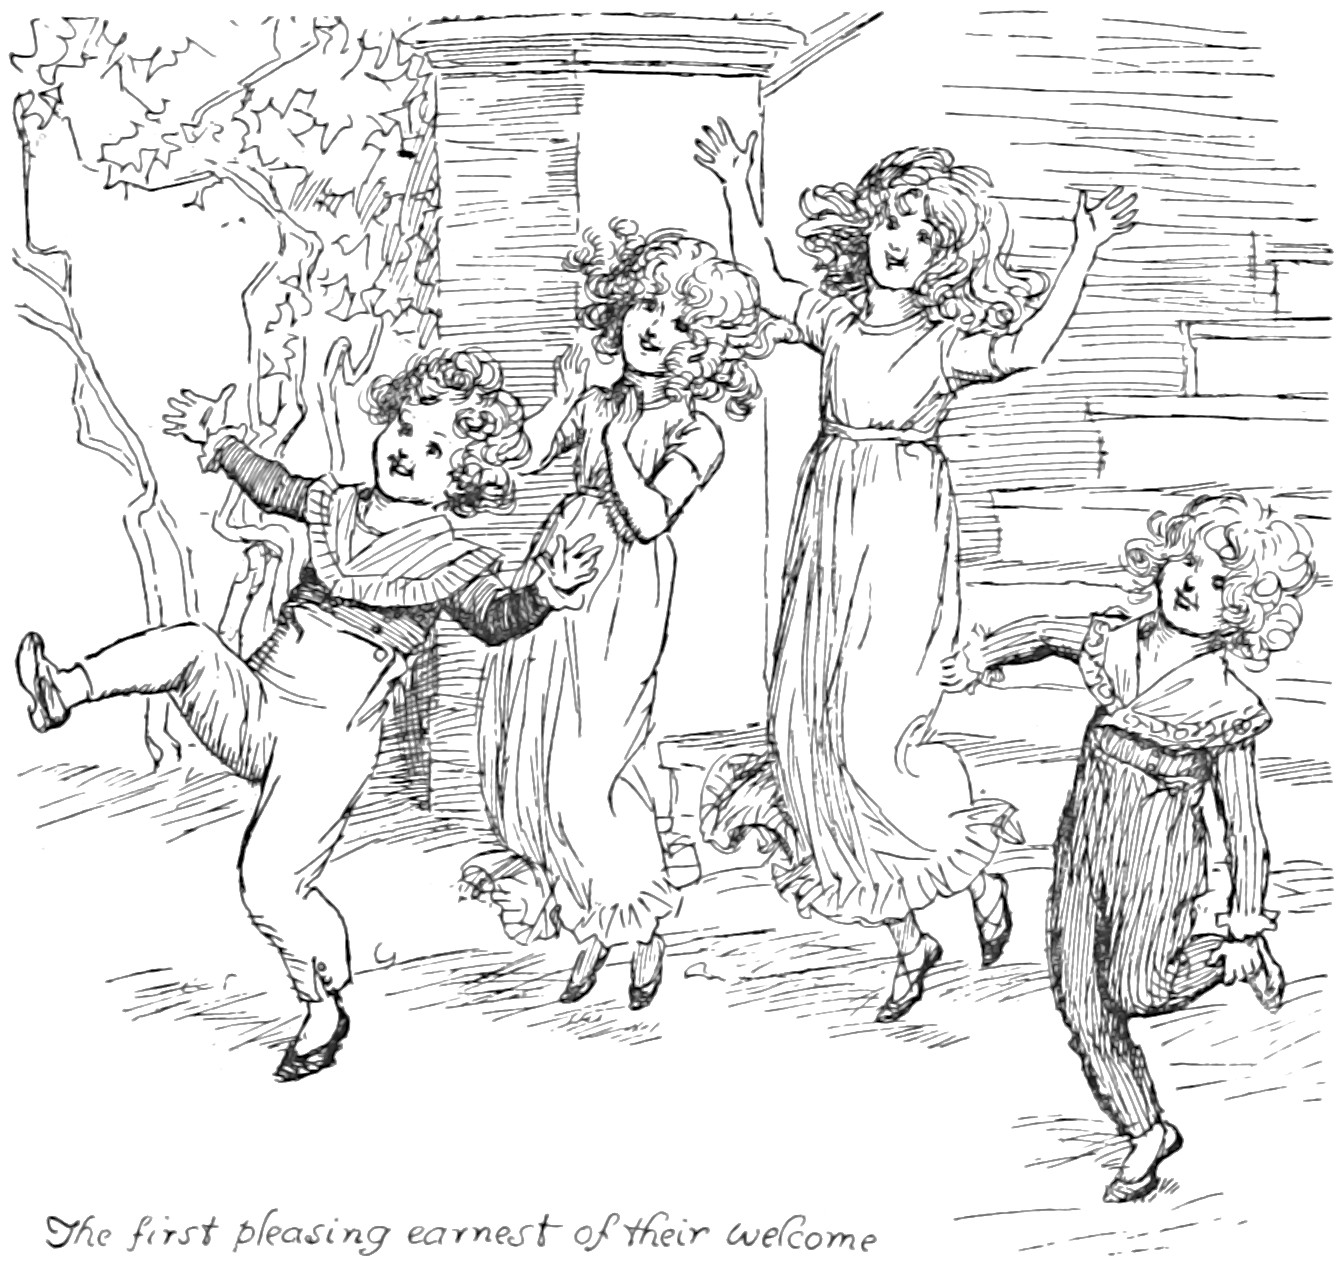
\includegraphics[width=.8\linewidth]{47top}
\captionlistentry{The first pleasing earnest of their welcome}
\end{figure}

\lettrine[lines=6,image=true,ante=`,loversize=.1,findent=2pt]{initials/chap47i}{} have been thinking it over again, Elizabeth,' said her uncle, as they drove from the town; »and really, upon serious consideration, I am much more inclined than I was to judge as your eldest sister does of the matter. It appears to me so very unlikely that any young man should form such a design against a girl who is by no means unprotected or friendless, and who was actually staying in his Colonel's family, that I am strongly inclined to hope the best. Could he expect that her friends would not step forward? Could he expect to be noticed again by the regiment, after such an affront to Colonel Forster? His temptation is not adequate to the risk.«

»Do you really think so?« cried Elizabeth, brightening up for a moment.

»Upon my word,« said Mrs Gardiner, »I begin to be of your uncle's opinion. It is really too great a violation of decency, honour, and interest, for him to be guilty of it. I cannot think so very ill of Wickham. Can you, yourself, Lizzie, so wholly give him up, as to believe him capable of it?«

»Not perhaps of neglecting his own interest. But of every other neglect I can believe him capable. If, indeed, it should be so! But I dare not hope it. Why should they not go on to Scotland, if that had been the case?«

»In the first place,« replied Mr Gardiner, »there is no absolute proof that they are not gone to Scotland.«

»Oh, but their removing from the chaise into a hackney coach is such a presumption! And, besides, no traces of them were to be found on the Barnet road.«

»Well, then,—supposing them to be in London—they may be there, though for the purpose of concealment, for no more exceptionable purpose. It is not likely that money should be very abundant on either side; and it might strike them that they could be more economically, though less expeditiously, married in London, than in Scotland.«

»But why all this secrecy? Why any fear of detection? Why must their marriage be private? Oh, no, no—this is not likely. His most particular friend, you see by Jane's account, was persuaded of his never intending to marry her. Wickham will never marry a woman without some money. He cannot afford it. And what claims has Lydia, what attractions has she beyond youth, health, and good humour, that could make him for her sake forego every chance of benefiting himself by marrying well? As to what restraint the apprehensions of disgrace in the corps might throw on a dishonourable elopement with her, I am not able to judge; for I know nothing of the effects that such a step might produce. But as to your other objection, I am afraid it will hardly hold good. Lydia has no brothers to step forward; and he might imagine, from my father's behaviour, from his indolence and the little attention he has ever seemed to give to what was going forward in his family, that \textit{he} would do as little and think as little about it, as any father could do, in such a matter.«

»But can you think that Lydia is so lost to everything but love of him, as to consent to live with him on any other terms than marriage?«

»It does seem, and it is most shocking, indeed,« replied Elizabeth, with tears in her eyes, »that a sister's sense of decency and virtue in such a point should admit of doubt. But, really, I know not what to say. Perhaps I am not doing her justice. But she is very young: she has never been taught to think on serious subjects; and for the last half year, nay, for a twelvemonth, she has been given up to nothing but amusement and vanity. She has been allowed to dispose of her time in the most idle and frivolous manner, and to adopt any opinions that came in her way. Since the ——shire were first quartered in Meryton, nothing but love, flirtation, and officers, have been in her head. She has been doing everything in her power, by thinking and talking on the subject, to give greater—what shall I call it?—susceptibility to her feelings; which are naturally lively enough. And we all know that Wickham has every charm of person and address that can captivate a woman.«

»But you see that Jane,« said her aunt, »does not think so ill of Wickham, as to believe him capable of the attempt.«

»Of whom does Jane ever think ill? And who is there, whatever might be their former conduct, that she would believe capable of such an attempt, till it were proved against them? But Jane knows, as well as I do, what Wickham really is. We both know that he has been profligate in every sense of the word; that he has neither integrity nor honour; that he is as false and deceitful as he is insinuating.«

»And do you really know all this?« cried Mrs Gardiner, whose curiosity as to the mode of her intelligence was all alive.

»I do, indeed,« replied Elizabeth, colouring. »I told you the other day of his infamous behaviour to Mr Darcy; and you, yourself, when last at Longbourn, heard in what manner he spoke of the man who had behaved with such forbearance and liberality towards him. And there are other circumstances which I am not at liberty—which it is not worth while to relate; but his lies about the whole Pemberley family are endless. From what he said of Miss Darcy, I was thoroughly prepared to see a proud, reserved, disagreeable girl. Yet he knew to the contrary himself. He must know that she was as amiable and unpretending as we have found her.«

»But does Lydia know nothing of this? can she be ignorant of what you and Jane seem so well to understand?«

»Oh, yes!—that, that is the worst of all. Till I was in Kent, and saw so much both of Mr Darcy and his relation Colonel Fitzwilliam, I was ignorant of the truth myself. And when I returned home the ——shire was to leave Meryton in a week or fortnight's time. As that was the case, neither Jane, to whom I related the whole, nor I, thought it necessary to make our knowledge public; for of what use could it apparently be to anyone, that the good opinion, which all the neighbourhood had of him, should then be overthrown? And even when it was settled that Lydia should go with Mrs Forster, the necessity of opening her eyes to his character never occurred to me. That \textit{she} could be in any danger from the deception never entered my head. That such a consequence as \textit{this} should ensue, you may easily believe was far enough from my thoughts.«

»When they all removed to Brighton, therefore, you had no reason, I suppose, to believe them fond of each other?«

»Not the slightest. I can remember no symptom of affection on either side; and had anything of the kind been perceptible, you must be aware that ours is not a family on which it could be thrown away. When first he entered the corps, she was ready enough to admire him; but so we all were. Every girl in or near Meryton was out of her senses about him for the first two months: but he never distinguished \textit{her} by any particular attention; and, consequently, after a moderate period of extravagant and wild admiration, her fancy for him gave way, and others of the regiment, who treated her with more distinction, again became her favourites.«

It may be easily believed, that however little of novelty could be added to their fears, hopes, and conjectures, on this interesting subject by its repeated discussion, no other could detain them from it long, during the whole of the journey. From Elizabeth's thoughts it was never absent. Fixed there by the keenest of all anguish, self-reproach, she could find no interval of ease or forgetfulness.

They travelled as expeditiously as possible; and sleeping one night on the road, reached Longbourn by dinnertime the next day. It was a comfort to Elizabeth to consider that Jane could not have been wearied by long expectations.

The little Gardiners, attracted by the sight of a chaise, were standing on the steps of the house, as they entered the paddock; and when the carriage drove up to the door, the joyful surprise that lighted up their faces and displayed itself over their whole bodies, in a variety of capers and frisks, was the first pleasing earnest of their welcome.

Elizabeth jumped out; and after giving each of them a hasty kiss, hurried into the vestibule, where Jane, who came running downstairs from her mother's apartment, immediately met her.

Elizabeth, as she affectionately embraced her, whilst tears filled the eyes of both, lost not a moment in asking whether anything had been heard of the fugitives.

»Not yet,« replied Jane. »But now that my dear uncle is come, I hope everything will be well.«

»Is my father in town?«

»Yes, he went on Tuesday, as I wrote you word.«

»And have you heard from him often?«

»We have heard only once. He wrote me a few lines on Wednesday, to say that he had arrived in safety, and to give me his directions, which I particularly begged him to do. He merely added, that he should not write again, till he had something of importance to mention.«

»And my mother—how is she? How are you all?«

»My mother is tolerably well, I trust; though her spirits are greatly shaken. She is upstairs, and will have great satisfaction in seeing you all. She does not yet leave her dressing-room. Mary and Kitty, thank Heaven! are quite well.«

»But you—how are you?« cried Elizabeth. »You look pale. How much you must have gone through!«

Her sister, however, assured her of her being perfectly well; and their conversation, which had been passing while Mr and Mrs Gardiner were engaged with their children, was now put an end to by the approach of the whole party. Jane ran to her uncle and aunt, and welcomed and thanked them both, with alternate smiles and tears.

When they were all in the drawing-room, the questions which Elizabeth had already asked were of course repeated by the others, and they soon found that Jane had no intelligence to give. The sanguine hope of good, however, which the benevolence of her heart suggested, had not yet deserted her; she still expected that it would all end well, and that every morning would bring some letter, either from Lydia or her father, to explain their proceedings, and, perhaps, announce the marriage.

Mrs Bennet, to whose apartment they all repaired, after a few minutes' conversation together, received them exactly as might be expected; with tears and lamentations of regret, invectives against the villainous conduct of Wickham, and complaints of her own sufferings and ill-usage; blaming everybody but the person to whose ill-judging indulgence the errors of her daughter must be principally owing.

»If I had been able,« said she, »to carry my point in going to Brighton with all my family, \textit{this} would not have happened: but poor dear Lydia had nobody to take care of her. Why did the Forsters ever let her go out of their sight? I am sure there was some great neglect or other on their side, for she is not the kind of girl to do such a thing, if she had been well looked after. I always thought they were very unfit to have the charge of her; but I was over-ruled, as I always am. Poor, dear child! And now here's Mr Bennet gone away, and I know he will fight Wickham, wherever he meets him, and then he will be killed, and what is to become of us all? The Collinses will turn us out, before he is cold in his grave; and if you are not kind to us, brother, I do not know what we shall do.«

They all exclaimed against such terrific ideas; and Mr Gardiner, after general assurances of his affection for her and all her family, told her that he meant to be in London the very next day, and would assist Mr Bennet in every endeavour for recovering Lydia.

»Do not give way to useless alarm,« added he: »though it is right to be prepared for the worst, there is no occasion to look on it as certain. It is not quite a week since they left Brighton. In a few days more, we may gain some news of them; and till we know that they are not married, and have no design of marrying, do not let us give the matter over as lost. As soon as I get to town, I shall go to my brother, and make him come home with me to Gracechurch Street, and then we may consult together as to what is to be done.«

»Oh, my dear brother,« replied Mrs Bennet, »that is exactly what I could most wish for. And now do, when you get to town, find them out, wherever they may be; and if they are not married already, \textit{make} them marry. And as for wedding clothes, do not let them wait for that, but tell Lydia she shall have as much money as she chooses to buy them, after they are married. And, above all things, keep Mr Bennet from fighting. Tell him what a dreadful state I am in—that I am frightened out of my wits; and have such tremblings, such flutterings all over me, such spasms in my side, and pains in my head, and such beatings at my heart, that I can get no rest by night nor by day. And tell my dear Lydia not to give any directions about her clothes till she has seen me, for she does not know which are the best warehouses. Oh, brother, how kind you are! I know you will contrive it all.«

But Mr Gardiner, though he assured her again of his earnest endeavours in the cause, could not avoid recommending moderation to her, as well in her hopes as her fears; and after talking with her in this manner till dinner was on table, they left her to vent all her feelings on the housekeeper, who attended in the absence of her daughters.

Though her brother and sister were persuaded that there was no real occasion for such a seclusion from the family, they did not attempt to oppose it; for they knew that she had not prudence enough to hold her tongue before the servants, while they waited at table, and judged it better that \textit{one} only of the household, and the one whom they could most trust, should comprehend all her fears and solicitude on the subject.

In the dining-room they were soon joined by Mary and Kitty, who had been too busily engaged in their separate apartments to make their appearance before. One came from her books, and the other from her toilette. The faces of both, however, were tolerably calm; and no change was visible in either, except that the loss of her favourite sister, or the anger which she had herself incurred in the business, had given something more of fretfulness than usual to the accents of Kitty. As for Mary, she was mistress enough of herself to whisper to Elizabeth, with a countenance of grave reflection, soon after they were seated at table,—

»This is a most unfortunate affair, and will probably be much talked of. But we must stem the tide of malice, and pour into the wounded bosoms of each other the balm of sisterly consolation.«

Then perceiving in Elizabeth no inclination of replying, she added, »Unhappy as the event must be for Lydia, we may draw from it this useful lesson:—that loss of virtue in a female is irretrievable, that one false step involves her in endless ruin, that her reputation is no less brittle than it is beautiful, and that she cannot be too much guarded in her behaviour towards the undeserving of the other sex.«

Elizabeth lifted up her eyes in amazement, but was too much oppressed to make any reply. Mary, however, continued to console herself with such kind of moral extractions from the evil before them.

In the afternoon, the two elder Miss Bennets were able to be for half an hour by themselves; and Elizabeth instantly availed herself of the opportunity of making any inquiries which Jane was equally eager to satisfy. After joining in general lamentations over the dreadful sequel of this event, which Elizabeth considered as all but certain, and Miss Bennet could not assert to be wholly impossible, the former continued the subject by saying, »But tell me all and everything about it which I have not already heard. Give me further particulars. What did Colonel Forster say? Had they no apprehension of anything before the elopement took place? They must have seen them together for ever.«

»Colonel Forster did own that he had often suspected some partiality, especially on Lydia's side, but nothing to give him any alarm. I am so grieved for him. His behaviour was attentive and kind to the utmost. He \textit{was} coming to us, in order to assure us of his concern, before he had any idea of their not being gone to Scotland: when that apprehension first got abroad, it hastened his journey.«

»And was Denny convinced that Wickham would not marry? Did he know of their intending to go off? Had Colonel Forster seen Denny himself?«

»Yes; but when questioned by \textit{him}, Denny denied knowing anything of their plan, and would not give his real opinion about it. He did not repeat his persuasion of their not marrying, and from \textit{that} I am inclined to hope he might have been misunderstood before.«

»And till Colonel Forster came himself, not one of you entertained a doubt, I suppose, of their being really married?«

»How was it possible that such an idea should enter our brains? I felt a little uneasy—a little fearful of my sister's happiness with him in marriage, because I knew that his conduct had not been always quite right. My father and mother knew nothing of that; they only felt how imprudent a match it must be. Kitty then owned, with a very natural triumph on knowing more than the rest of us, that in Lydia's last letter she had prepared her for such a step. She had known, it seems, of their being in love with each other many weeks.«

»But not before they went to Brighton?«

»No, I believe not.«

»And did Colonel Forster appear to think ill of Wickham himself? Does he know his real character?«

»I must confess that he did not speak so well of Wickham as he formerly did. He believed him to be imprudent and extravagant; and since this sad affair has taken place, it is said that he left Meryton greatly in debt: but I hope this may be false.«

»Oh, Jane, had we been less secret, had we told what we knew of him, this could not have happened!«

»Perhaps it would have been better,« replied her sister.

»But to expose the former faults of any person, without knowing what their present feelings were, seemed unjustifiable.«

»We acted with the best intentions.«

»Could Colonel Forster repeat the particulars of Lydia's note to his wife?«

»He brought it with him for us to see.«

Jane then took it from her pocket-book, and gave it to Elizabeth. These were the contents:—


\begin{quotation}
\noindent My dear Harriet,\\

\indent You will laugh when you know where I am gone, and I cannot help laughing myself at your surprise to-morrow morning, as soon as I am missed. I am going to Gretna Green, and if you cannot guess with who, I shall think you a simpleton, for there is but one man in the world I love, and he is an angel. I should never be happy without him, so think it no harm to be off. You need not send them word at Longbourn of my going, if you do not like it, for it will make the surprise the greater when I write to them, and sign my name Lydia Wickham. What a good joke it will be! I can hardly write for laughing. Pray make my excuses to Pratt for not keeping my engagement, and dancing with him to-night. Tell him I hope he will excuse me when he knows all, and tell him I will dance with him at the next ball we meet with great pleasure. I shall send for my clothes when I get to Longbourn; but I wish you would tell Sally to mend a great slit in my worked muslin gown before they are packed up. Good-bye. Give my love to Colonel Forster. I hope you will drink to our good journey.

\begin{flushright}
Your affectionate friend,\\
\textsc{Lydia Bennet.}
\end{flushright}
\end{quotation}


»Oh, thoughtless, thoughtless Lydia!« cried Elizabeth when she had finished it. »What a letter is this, to be written at such a moment! But at least it shows that \textit{she} was serious in the object of her journey. Whatever he might afterwards persuade her to, it was not on her side a \textit{scheme} of infamy. My poor father! how he must have felt it!«

»I never saw anyone so shocked. He could not speak a word for full ten minutes. My mother was taken ill immediately, and the whole house in such confusion!«

»Oh, Jane,« cried Elizabeth, »was there a servant belonging to it who did not know the whole story before the end of the day?«

»I do not know: I hope there was. But to be guarded at such a time is very difficult. My mother was in hysterics; and though I endeavoured to give her every assistance in my power, I am afraid I did not do so much as I might have done. But the horror of what might possibly happen almost took from me my faculties.«

»Your attendance upon her has been too much for you. You do not look well. Oh that I had been with you! you have had every care and anxiety upon yourself alone.«

»Mary and Kitty have been very kind, and would have shared in every fatigue, I am sure, but I did not think it right for either of them. Kitty is slight and delicate, and Mary studies so much that her hours of repose should not be broken in on. My aunt Philips came to Longbourn on Tuesday, after my father went away; and was so good as to stay till Thursday with me. She was of great use and comfort to us all, and Lady Lucas has been very kind: she walked here on Wednesday morning to condole with us, and offered her services, or any of her daughters, if they could be of use to us.«

»She had better have stayed at home,« cried Elizabeth: »perhaps she \textit{meant} well, but, under such a misfortune as this, one cannot see too little of one's neighbours. Assistance is impossible; condolence, insufferable. Let them triumph over us at a distance, and be satisfied.«

She then proceeded to inquire into the measures which her father had intended to pursue, while in town, for the recovery of his daughter.

»He meant, I believe,« replied Jane, »to go to Epsom, the place where they last changed horses, see the postilions, and try if anything could be made out from them. His principal object must be to discover the number of the hackney coach which took them from Clapham. It had come with a fare from London; and as he thought the circumstance of a gentleman and lady's removing from one carriage into another might be remarked, he meant to make inquiries at Clapham. If he could anyhow discover at what house the coachman had before set down his fare, he determined to make inquiries there, and hoped it might not be impossible to find out the stand and number of the coach. I do not know of any other designs that he had formed; but he was in such a hurry to be gone, and his spirits so greatly discomposed, that I had difficulty in finding out even so much as this.«